\begin{center}\textbf{\color{red}LUYỆN TẬP}\\
	\textbf{Bài 7. GIA TỐC - CHUYỂN ĐỘNG THẲNG BIẾN ĐỔI ĐỀU}
\end{center}
\section{TRẮC NGHIỆM}
\Opensolutionfile{ans}[ans/BAI7-TN]
% ===================================================================
\begin{ex}
	Một xe máy đang đứng yên, sau đó khởi động và bắt đầu tăng tốc. Nếu chọn chiều dương cùng  chiều chuyển động của xe, nhận xét nào sau đây là đúng? 
	\choice
	{$a<0$, $v<0$}
	{$a>0$, $v<0$}
	{\True $a>0$, $v>0$}
	{$a<0$, $v>0$}
	\loigiai{}
\end{ex}
% ===================================================================
\begin{ex}
	Gia tốc là đại lượng
	\choice
	{\True vector, đặc trưng cho sự biến thiên nhanh hay chậm của vận tốc}
	{vô hướng, đặc trưng cho tính chất nhanh hay chậm của chuyển động}
	{vector, đặc trưng cho tính chất nhanh hay chậm của chuyển động}
	{vô hướng, đặc trưng cho tính sự biến thiên nhanh hay chậm của vận tốc}
	\loigiai{}
\end{ex}
% ===================================================================
\begin{ex}
	Công thức liên hệ giữa độ dịch chuyển, vận tốc và gia tốc của chuyển động nhanh dần đều là
	\choice
	{$v^2-v^2_0=ad$}
	{\True $v^2-v^2_0=2ad$}
	{$v-v_0=2ad$}
	{$v^2_0-v^2=2ad$}
	\loigiai{}
\end{ex}
% ===================================================================
\begin{ex}
	Trong các phương trình mô tả vận tốc $v\ \left(\si{\meter/\second}\right)$ của vật theo thời gian $t\ \left(\si{\second}\right)$ dưới đây, phương trình nào mô tả chuyển động thẳng biến đổi đều?
	\choice
	{$v=7$}
	{$v=6t^2+2t-2$}
	{\True $v=5t-4$}
	{$v=6t^2-2$}
	\loigiai{}
\end{ex}
% ===================================================================
\begin{ex}
Cho các đồ thị độ dịch chuyển - thời gian $\left(d-t\right)$ và vận tốc - thời gian $\left(v-t\right)$ như hình bên dưới. Đồ thị ứng với chuyển động thẳng biến đổi đều là
\begin{center}
	\begin{tabular}{M{4cm}M{4cm}M{4cm}M{4cm}}
		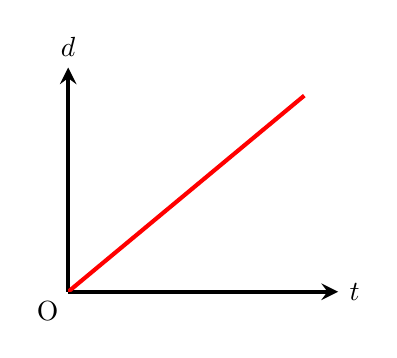
\begin{tikzpicture}  
			\begin{axis}[  ultra thick,scale=0.5,
				xmin=0,  
				xmax=4,  
				ymin=0,  
				ymax=4, 
				samples=300,
				yticklabels=\empty,
				xticklabels=\empty,
				xtick=\empty,
				ytick=\empty,
				axis lines=center, 
				xlabel=$t$, 		ylabel=$d$,
				every axis y label/.style={at=(current axis.above origin),anchor=south},  
				every axis x label/.style={at=(current axis.right of origin),anchor=west},  ]
				\addplot [line width=1.5pt, red, smooth, domain=0:3.5] {x};  
				\coordinate (O) at (0,0);
			\end{axis}  
			\node[below left] at (O) {O};
		\end{tikzpicture}&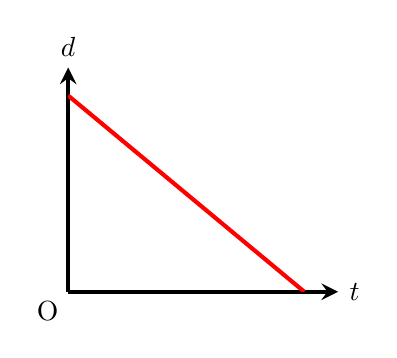
\begin{tikzpicture}  
		\begin{axis}[  ultra thick,scale=0.5,
			xmin=0,  
			xmax=4,  
			ymin=0,  
			ymax=4, 
			samples=300,
			yticklabels=\empty,
			xticklabels=\empty,
			xtick=\empty,
			ytick=\empty,
			axis lines=center, 
			xlabel=$t$, 		ylabel=$d$,
			every axis y label/.style={at=(current axis.above origin),anchor=south},  
			every axis x label/.style={at=(current axis.right of origin),anchor=west},  ]
			\addplot [line width=1.5pt, red, smooth, domain=0:3.5] {3.5-x};  
			\coordinate (O) at (0,0);
		\end{axis}  
		\node[below left] at (O) {O};
		\end{tikzpicture}&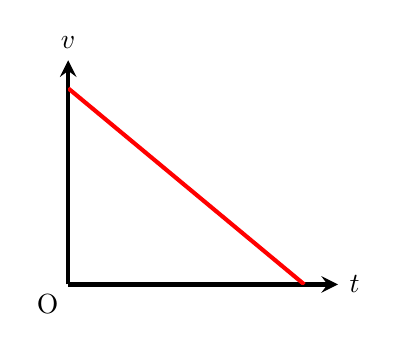
\begin{tikzpicture}  
		\begin{axis}[  ultra thick,scale=0.5,
			xmin=0,  
			xmax=4,  
			ymin=0,  
			ymax=4, 
			samples=300,
			yticklabels=\empty,
			xticklabels=\empty,
			xtick=\empty,
			ytick=\empty,
			axis lines=center, 
			xlabel=$t$, 		ylabel=$v$,
			every axis y label/.style={at=(current axis.above origin),anchor=south},  
			every axis x label/.style={at=(current axis.right of origin),anchor=west},  ]
			\addplot [line width=1.5pt, red, smooth, domain=0:3.5] {3.5-x};  
			\coordinate (O) at (0,0);
		\end{axis}  
		\node[below left] at (O) {O};
		\end{tikzpicture}&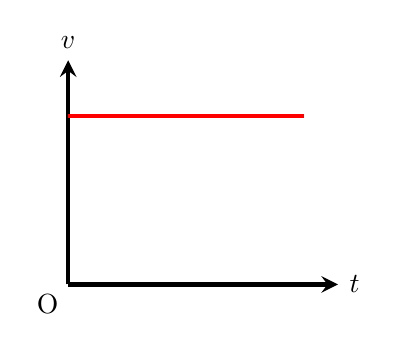
\begin{tikzpicture}  
		\begin{axis}[  ultra thick,scale=0.5,
			xmin=0,  
			xmax=4,  
			ymin=0,  
			ymax=4, 
			samples=300,
			yticklabels=\empty,
			xticklabels=\empty,
			xtick=\empty,
			ytick=\empty,
			axis lines=center, 
			xlabel=$t$, 		ylabel=$v$,
			every axis y label/.style={at=(current axis.above origin),anchor=south},  
			every axis x label/.style={at=(current axis.right of origin),anchor=west},  ]
			\addplot [line width=1.5pt, red, smooth, domain=0:3.5] {3};  
			\coordinate (O) at (0,0);
		\end{axis}  
		\node[below left] at (O) {O};
		\end{tikzpicture}\\
		Hình 1&Hình 2&Hình 3&Hình 4
	\end{tabular}
\end{center}	
	\choice
	{Hình 1 và Hình 4}
	{Hình 2 và Hình 3}
	{\True Hình 3}
	{Hình 1}
	\loigiai{}
\end{ex}
% ===================================================================
\begin{ex}
	Chọn phát biểu \textbf{sai}.
	\choice
	{Gia tốc của vật chuyển động thẳng biến đổi đều có độ lớn không đổi}
	{\True Trong chuyển động thẳng biến đổi đều, quãng đường vật đi được trong những khoảng thời gian bằng nhau thì bằng nhau}
	{Vận tốc tức thời của vật chuyển động thẳng biến đổi đều có độ lớn tăng hoặc giảm đều theo thời gian}
	{Vectơ gia tốc của vật chuyển động thẳng biến đổi đều có thể cùng chiều hoặc ngược chiều với vectơ vận tốc}
	\loigiai{}
\end{ex}
% ===================================================================
\begin{ex}
	Một ô tô đang chạy với tốc độ $\SI{72}{\kilo\meter/\hour}$ thì hãm phanh, chạy chậm dần đều sau $\SI{10}{\second}$ tốc độ giảm còn $\SI{10}{\meter/\second}$. Thời gian từ lúc hãm phanh đến lúc dừng lại là
	\choice
	{$\SI{30}{\second}$}
	{\True $\SI{20}{\second}$}
	{$\SI{12}{\second}$}
	{$\SI{40}{\second}$}
	\loigiai{}
\end{ex}
% ===================================================================
\begin{ex}
Trong chuyển động thẳng nhanh dần đều	
	\choice
	{$a<0$}
	{\True $v\cdot a>0$}
	{$ a>0$}
	{$v\cdot a<0$}
	\loigiai{}
\end{ex}
% ===================================================================
\begin{ex}
Một ô tô đang chạy với tốc độ $\SI{12}{\meter/\second}$ trên một đoạn đường thẳng thì người lái xe tăng
ga cho ôtô chạy nhanh dần đều. Sau $\SI{15}{\second}$ ôtô đạt tốc độ $\SI{15}{\meter/\second}$. Quãng đường của ô tô
đi được sau $\SI{5}{\second}$ kể từ khi tăng ga là	
	\choice
	{$\SI{72.5}{\meter}$}
	{$\SI{65}{\meter}$}
	{$\SI{57.5}{\meter}$}
	{\True $\SI{62.5}{\meter}$}
	\loigiai{}
\end{ex}
% ===================================================================
\begin{ex}
	Một đoàn tàu đang đứng yên  thì bắt đầu tăng tốc chuyển động thẳng nhanh dần đều. Trong khoảng thời gian tăng tốc từ $\SI{21.6}{\kilo\meter/\hour}$ đến $\SI{36}{\kilo\meter/\hour}$, tàu đi được $\SI{64}{\meter}$. Gia tốc của tàu và quãng đường tàu đi được kể từ lúc bắt đầu chuyển động đến khi đạt tốc độ $\SI{36}{\kilo\meter/\hour}$ là
	\choice
	{$a=\SI{-0.7}{\meter/\second^2}$, $s=\SI{200}{\meter}$}
	{$a=\SI{-0.5}{\meter/\second^2}$, $s=\SI{110}{\meter}$}
	{\True $a=\SI{0.5}{\meter/\second^2}$, $s=\SI{100}{\meter}$}
	{$a=\SI{-0.5}{\meter/\second^2}$, $s=\SI{100}{\meter}$}
	\loigiai{}
\end{ex}

% ===================================================================
\begin{ex}
Hình bên mô tả đồ thị $\left(v-t\right)$ của bốn xe ô tô A, B, C, D. Nhận định nào sau đây là đúng?
\begin{center}
	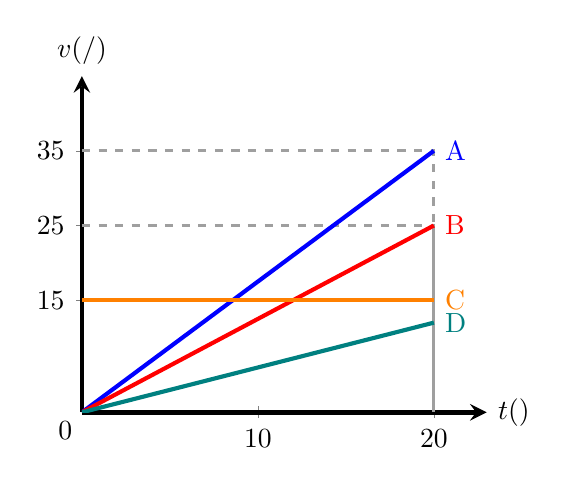
\begin{tikzpicture}  
		\begin{axis}[  ultra thick,scale=0.75,
			xmin=0,  
			xmax=23,  
			xtick={0,10,20},
			ytick={0,15,25,35},
			ymin=0,  
			ymax=45, 
			samples=300,
			axis lines=center, 
			xlabel=$\xsi{t}{\left(\si{\second}\right)}$, 		ylabel=$\xsi{v}{\left(\si{\meter/\second}\right)}$,
			every axis y label/.style={at=(current axis.above origin),anchor=south},  
			every axis x label/.style={at=(current axis.right of origin),anchor=west},  ]
			\draw[dashed, line width=1pt, gray!75!white] (axis cs: 0,35)--(axis cs: 20,35)--(axis cs: 20,0);
			\draw[dashed, line width=1pt, gray!75!white] (axis cs: 0,25)--(axis cs: 20,25)--(axis cs: 20,0);
			\addplot [line width=1.5pt, blue, smooth, domain=0:20] {1.75*x} node[right] {A};
			\addplot [line width=1.5pt, red, smooth, domain=0:20] {1.25*x} node[right] {B}; 
			\addplot [line width=1.5pt,teal , smooth, domain=0:20] {0.6*x} node[right] {D}; 
			\addplot [line width=1.5pt, orange, smooth, domain=0:20] {15} node[right] {C};
			\coordinate (O) at (0,0);
		\end{axis}  
		\node[below left] at (O) {0};
	\end{tikzpicture}
\end{center}	
	\choice
	{\True Xe C chuyển động đều, còn các xe còn lại là chuyển động biến đổi đều}
	{Chỉ có xe A và B chuyển động biến đồi đều, xe C chuyển động đều}
	{Gia tốc xe A có độ lớn nhỏ hơn gia tốc xe D}
	{Xe D chuyển động biến đổi đều, xe C chuyển động đều}
	\loigiai{}
\end{ex}
% ===================================================================
\begin{ex}
	Một vật chuyển động dọc theo trục $Ox$ có phương trình chuyển động $x=3-4t+2t^2\ \left(\si{\meter};\si{\second}\right)$. Biểu thức vận tốc của vật theo thời gian là
	\choice
	{$v=\xsi{2\left(t-2\right)}{\meter/\second}$}
	{$v=\xsi{2\left(t+2\right)}{\meter/\second}$}
	{\True $v=\xsi{4\left(t-1\right)}{\meter/\second}$}
	{$v=\xsi{2\left(t-1\right)}{\meter/\second}$}
	\loigiai{}
\end{ex}
% ===================================================================
\begin{ex}
Một vật chuyển động dọc theo trục $Ox$ có phương trình chuyển động $x=10t+5t^2\ \left(\si{\meter}; \si{\second}\right)$. Vận tốc của vật tại thời điểm $t=\SI{2}{\second}$ là	
	\choice
	{$\SI{40}{\meter/\second}$}
	{$\SI{20}{\meter/\second}$}
	{\True $\SI{30}{\meter/\second}$}
	{$\SI{26}{\meter/\second}$}
	\loigiai{}
\end{ex}
% ===================================================================
\begin{ex}
Phương trình chuyển động của một vật trên trục $Ox$ có dạng: $x=-2t^2+15t+10$.	Trong đó $t$ tính bằng giây, $x$ tính bằng mét. Vật này chuyển động
	\choice
	{nhanh dần đều rồi chậm dần đều theo chiều dương của trục $Ox$}
	{chậm dần đều rồi nhanh dần đều theo chiều âm của trục $Ox$}
	{nhanh dần đều rồi chậm dần đều theo chiều âm của trục $Ox$}
	{\True chậm dần đều theo chiều dương rồi nhanh dần đều theo chiều âm của trục $Ox$}
	\loigiai{}
\end{ex}
% ===================================================================
\begin{ex}
	\immini{Đồ thị vận tốc - thời gian của một vật chuyển động thẳng biến đổi trong 5 giây đầu tiên được cho như hình vẽ bên. Kết luận nào sau đây là đúng?
	\choice
	{\True Vật chuyển động chậm dần đều theo chiều âm với gia tốc $\SI{2}{\meter/\second^2}$}
	{Vật chuyển động thẳng đều theo chiều dương}
	{Vật chuyển động nhanh dần đều theo chiều dương với gia tốc $\SI{2}{\meter/\second^2}$}
	{Vật chuyển động nhanh dần đều theo chiều âm với gia tốc $\SI{-2}{\meter/\second^2}$}
	\loigiai{}}
	{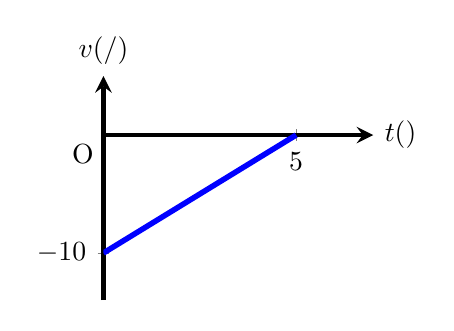
\begin{tikzpicture}  
			\begin{axis}[  ultra thick,scale=0.5,
				xmin=0,  
				xmax=7,  
				xtick={0,5},
				ytick={-10,0},
				ymin=-14,  
				ymax=5, 
				samples=300,
				axis lines=center, 
				xlabel=$\xsi{t}{\left(\si{\second}\right)}$, 		ylabel=$\xsi{v}{\left(\si{\meter/\second}\right)}$,
				every axis y label/.style={at=(current axis.above origin),anchor=south},  
				every axis x label/.style={at=(current axis.right of origin),anchor=west},  ]
				\addplot [line width=2pt, blue, smooth, domain=0:5] {-10+2*x};  
				\coordinate (O) at (axis cs: 0,0);
			\end{axis}  
			\node[below left] at (O) {O};
	\end{tikzpicture}}
\end{ex}
% ===================================================================
\begin{ex}
	Một vật chuyển động thẳng có đồ thị vận tốc theo thời gian như hình vẽ. Quãng đường vật đi được trong giai đoạn chậm dần đều là
	\begin{center}
		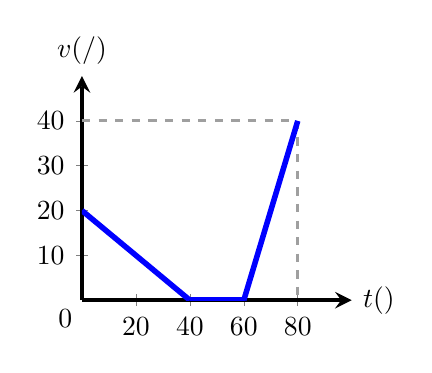
\begin{tikzpicture}  
			\begin{axis}[  ultra thick,scale=0.5,
				xmin=0,  
				xmax=100,  
				xtick={0,20,...,80},
				ytick={0,10,...,40},
				minor x tick num=0,
				minor y tick num=0,
				ymin=0,  
				ymax=50, 
				samples=300,
				axis lines=center, 
				xlabel=$\xsi{t}{\left(\si{\second}\right)}$, 		ylabel=$\xsi{v}{\left(\si{\meter/\second}\right)}$,
				every axis y label/.style={at=(current axis.above origin),anchor=south},  
				every axis x label/.style={at=(current axis.right of origin),anchor=west},  ]
				\draw[dashed, line width=1pt, gray!75!white] (axis cs: 0,40)--(axis cs: 80,40)--(axis cs: 80,0);
				\addplot [line width=2pt, blue, smooth, domain=0:40] {20-0.5*x};  
				\addplot [line width=2pt, blue, smooth, domain=40:60] {0}; 
				\addplot [line width=2pt, blue, smooth, domain=60:80] {2*(x-60)}; 
				\coordinate (O) at (0,0);
			\end{axis}  
			\node[below left] at (O) {0};
		\end{tikzpicture}
	\end{center}
	\choice
	{$\SI{600}{\meter}$}
	{$\SI{800}{\meter}$}
	{$\SI{200}{\meter}$}
	{\True $\SI{400}{\meter}$}
	\loigiai{}
\end{ex}
% ===================================================================
\begin{ex}
	Quan sát đồ thị $\left(v-t\right)$ như hình bên dưới của một vật đang chuyển động thẳng và cho biết quãng đường vật đi được trong khoảng thời gian nào lớn nhất?
	\begin{center}
		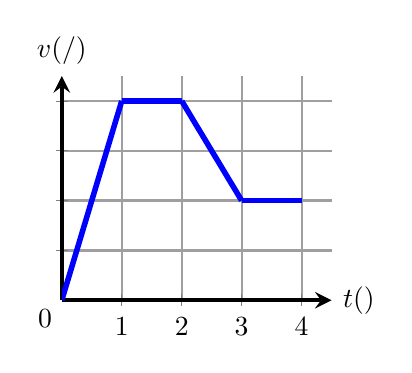
\begin{tikzpicture}  
			\begin{axis}[  ultra thick,scale=0.5,
				xmin=0,  
				xmax=4.5,  
				xtick={0,1,...,4},
				ytick={0,1,...,4},
				minor x tick num=0,
				minor y tick num=0,
				ymin=0,  
				ymax=4.5, 
				samples=300,
				yticklabels=\empty,
				axis lines=center, 
				grid style={step=1, line width =0.4pt, color=gray!40!white},
				grid=both, %giới hạn ô lưới
				major grid style={line width=0.8pt,gray!75!white},
				xlabel=$\xsi{t}{\left(\si{\second}\right)}$, 		ylabel=$\xsi{v}{\left(\si{\meter/\second}\right)}$,
				every axis y label/.style={at=(current axis.above origin),anchor=south},  
				every axis x label/.style={at=(current axis.right of origin),anchor=west},  ]
				\addplot [line width=2pt, blue, smooth, domain=0:1] {4*x};  
				\addplot [line width=2pt, blue, smooth, domain=1:2] {4}; 
				\addplot [line width=2pt, blue, smooth, domain=2:3] {4-2*(x-2)}; 
				\addplot [line width=2pt, blue, smooth, domain=3:4] {2}; 
				\coordinate (O) at (0,0);
			\end{axis}  
			\node[below left] at (O) {0};
		\end{tikzpicture}
	\end{center}
	\choice
	{Trong khoảng thời gian từ $\SI{0}{\second}$ đến $\SI{1}{\second}$}
	{\True Trong khoảng thời gian từ $\SI{1}{\second}$ đến $\SI{2}{\second}$}
	{Trong khoảng thời gian từ $\SI{2}{\second}$ đến $\SI{3}{\second}$}
	{Trong khoảng thời gian từ $\SI{3}{\second}$ đến $\SI{4}{\second}$}
	\loigiai{}
\end{ex}
% ===================================================================
\begin{ex}
Đồ thị vận tốc - thời gian của một vật chuyển động thẳng biến đổi đều được cho như hình vẽ bên. Biết rằng $v_1+v_2=\SI{15}{\meter/\second}$ và $t_2-t_1=\SI{6}{\second}$. Quãng đường vật đi được trong khoảng thời gian từ $t_1$ đến $t_2$ là
\begin{center}
	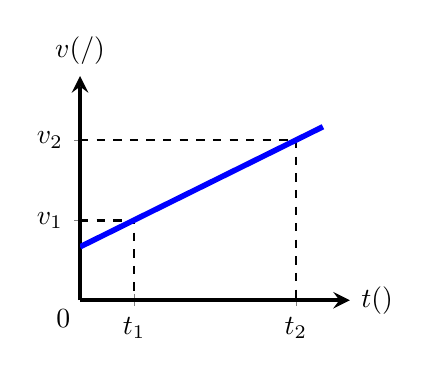
\begin{tikzpicture}  
		\begin{axis}[  ultra thick,scale=0.5,
			xmin=0,  
			xmax=10,  
			xtick={0,2,8},
			ytick={0,5,10},
			ymin=0,  
			ymax=14, 
			samples=300,
			yticklabels={0,$v_1$,$v_2$},
			xticklabels={0,$t_1$,$t_2$},
			axis lines=center, 
			xlabel=$\xsi{t}{\left(\si{\second}\right)}$, 		ylabel=$\xsi{v}{\left(\si{\meter/\second}\right)}$,
			every axis y label/.style={at=(current axis.above origin),anchor=south},  
			every axis x label/.style={at=(current axis.right of origin),anchor=west},  ]
			\draw[dashed, line width=1pt] (axis cs: 0,5)--(axis cs: 2,5)--(axis cs: 2,0);
			\draw[dashed, line width=1pt] (axis cs: 0,10)--(axis cs: 8,10)--(axis cs: 8,0);
			\addplot [line width=2pt, blue, smooth, domain=0:9] {10/3+5*x/6};  
			\coordinate (O) at (0,0);
		\end{axis}  
		\node[below left] at (O) {0};
	\end{tikzpicture}
\end{center}	
	\choice
	{$\SI{90}{\meter}$}
	{\True $\SI{45}{\meter}$}
	{$\SI{9}{\meter}$}
	{$\SI{540}{\meter}$}
	\loigiai{}
\end{ex}
% ===================================================================
\begin{ex}
	Một xe máy chạy đều trên một con đường thẳng với tốc độ $\SI{20}{\meter/\second}$ (vượt quá tốc độ) thì bị cảnh sát giao thông phát hiện. Chỉ sau $\SI{2}{\second}$ khi xe máy đi qua một cảnh sát, anh cảnh sát này bắt đầu đuổi theo với gia tốc không đổi và bằng $\SI{1.05}{\meter/\second^2}$. Thời điểm và vị trí anh cảnh sát đuổi kịp xe máy là
	\choice
	{\True sau $\SI{40}{\second}$ kể từ lúc anh cảnh sát xuất phát, cách vị trí xuất phát $\SI{840}{\meter}$}
	{sau $\SI{42}{\second}$ kể từ lúc anh cảnh sát xuất phát, cách vị trí xuất phát $\SI{840}{\meter}$}
	{sau $\SI{38}{\second}$ kể từ lúc anh cảnh sát xuất phát, cách vị trí xuất phát $\SI{760}{\meter}$}
	{sau $\SI{36}{\second}$ kể từ lúc anh cảnh sát xuất phát, cách vị trí xuất phát $\SI{760}{\meter}$}
	\loigiai{}
\end{ex}
% ===================================================================
\begin{ex}
	Hai xe A và B chuyển động cùng nhau vào hầm Thủ Thiêm dài $\SI{1490}{\meter}$. Xe A chuyển động với tốc độ ban đầu trước khi vào hầm là $\SI{60}{\kilo\meter/\hour}$ và chuyển động chậm dần đều với độ lớn gia tốc $\SI{144}{\kilo\meter/\hour^2}$, xe B chuyển động chậm dần đều với gia tốc $\SI{120}{\kilo\meter/\hour^2}$	từ lúc bắt đầu chạy vào hầm với tốc độ $\SI{55}{\kilo\meter/\hour}$. Nhận định nào sau đây là đúng về thời gian chuyển động của hai xe trong hầm?
	\choice
	{Hai xe đi hết hầm Thủ Thiêm cùng một khoảng thời gian}
	{Xe B ra khỏi hầm trước xe A}
	{\True Xe A ra khỏi hầm trước xe B}
	{Dữ liệu bài toán không đủ kết luận}
	\loigiai{}
\end{ex}
\Closesolutionfile{ans}
\section{TỰ LUẬN}
\Opensolutionfile{ans}[ans/BAI7-TL]
\setcounter{ex}{0}
% ======================================================================
\begin{ex}
	Quan sát đồ thị $\left(v-t\right)$ mô tả chuyển động thẳng của tàu hỏa trong hình bên dưới và trả lời các câu hỏi:
	\begin{center}
		\includegraphics[width=0.65\linewidth]{figs/BAI7-1}
	\end{center}
	\begin{enumerate}[label=\alph*)]
		\item Tại thời điểm nào, vận tôc tàu hỏa có giá trị lớn nhất?
		\item Vận tốc tàu hỏa không đổi trong khoảng thời gian nào?
		\item Tàu chuyển động thẳng nhanh dần đều trong khoảng thời gian nào?
	\end{enumerate}
	\loigiai{}
\end{ex}

% ======================================================================
\begin{ex}
	Đồ thị vận tốc $(v)$ – thời gian $(t)$ của một vật chuyển động thẳng được cho như hình bên. Xác định quãng đường vật đi được trong 6 giây đầu tiên và 6 giây cuối cùng của chuyển động.
	\begin{center}
		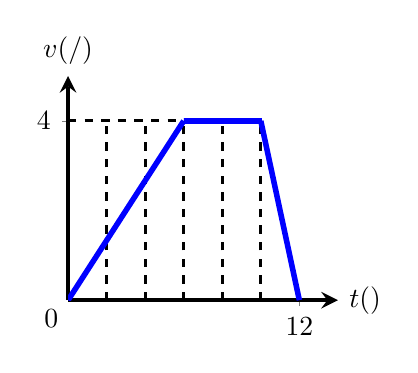
\begin{tikzpicture}  
			\begin{axis}[  ultra thick,scale=0.5,
				xmin=0,  
				xmax=14,  
				xtick={0,12},
				ytick={0,4},
				ymin=0,  
				ymax=5, 
				samples=300,
				axis lines=center,
				xlabel=$\xsi{t}{\left(\si{\second}\right)}$, 		ylabel=$\xsi{v}{\left(\si{\meter/\second}\right)}$,
				every axis y label/.style={at=(current axis.above origin),anchor=south},  
				every axis x label/.style={at=(current axis.right of origin),anchor=west},  ]
				\foreach \i in {2,4,...,10}{
				\edef\temp{\noexpand\draw[dashed, line width=1pt] (axis cs: \i,0)--(axis cs: \i,4);}
				\temp
				}
				\draw[dashed, line width=1pt] (axis cs: 0,4)--(axis cs: 10,4);
				\draw[dashed, line width=1pt] (axis cs: 0,40)--(axis cs: 80,40)--(axis cs: 80,0);
				\addplot [line width=2pt, blue, smooth, domain=0:6] {2*x/3};  
				\addplot [line width=2pt, blue, smooth, domain=6:10] {4}; 
				\addplot [line width=2pt, blue, smooth, domain=10:12] {4-2*(x-10)}; 
				\coordinate (O) at (0,0);
			\end{axis}  
			\node[below left] at (O) {0};
		\end{tikzpicture}
	\end{center}
	\loigiai{}
\end{ex}
% ======================================================================
\begin{ex}
	Một người đạp xe trên đường thẳng với tốc độ $\SI{4}{\meter/\second}$, bóp thắng để giảm tốc với gia tốc có độ lớn không đổi là $\SI{0.5}{\meter/\second^2}$. Xác định thời gian và quãng đường xe đi được từ khi bóp thắng đến khi dừng lại.
	\loigiai{}
\end{ex}
% ======================================================================
\begin{ex}
	Một ô tô chuyễn động chầm dần đều, trong $\SI{8.5}{\second}$ đi được quãng đường $\SI{40.0}{\meter}$ với vận tốc cuối cùng là $\SI{2.80}{\meter/\second}$.
	\begin{enumerate}[label=\alph*)]
		\item Tìm độ lớn vận tốc ban đầu của xe.
		\item Tìm gia tốc của xe.
	\end{enumerate}
	\loigiai{}
\end{ex}
% ======================================================================
\begin{ex}
Tại hiện trường một vụ tai nạn trên đường quốc lộ ngoài đô thị, cảnh sát phát hiện vết trượt kéo dài $\SI{50}{\meter}$. Qua các đo đạc trên mặt đường, cảnh sát kết luận gia tốc của ô tô trong quá trình giảm tốc có độ lớn $\SI{6.5}{\meter/\second^2}$. Nếu tốc độ giới hạn trên làn đường được quy định là $\SI{80}{\kilo\meter/\hour}$ thì ô tô này có vượt quá tốc độ cho phép không? Giả sử trong quá trình giảm tốc, ô tô chuyển động chậm dần đều.
	\loigiai{}
\end{ex}
% ======================================================================
\begin{ex}
	Một ô tô đang đi trên đường thẳng với tốc độ $v$ thì trước mặt ô tô đột ngột xuất hiện một mối nguy hiểm. Trong khoảng thời gian từ khi mối nguy xuất hiện đến khi phanh hoạt động, ô tô chuyển động được quãng đường $\SI{29.3}{\meter}$. Khi phanh hoạt động làm bánh xe ngừng quay, các bánh xe của ô tô để lại vết trượt dài $\SI{12.8}{\meter}$ trên đường, như minh hoạ trong hình bên dưới.
	\begin{center}
		\includegraphics[width=0.5\linewidth]{figs/BAI7-2}
	\end{center}
	Người ta ước tính rằng trong quá trình trượt, ô tô giảm tốc với gia tốc có độ lớn là $\SI{8.33}{\meter/\second^2}$. Xác định:
	\begin{enumerate}[label=\alph*)]
		\item Tốc độ $v$ của ô tô trước khi hãm phanh.
		\item Khoảng thời gian từ khi nguy hiểm xuất hiện đến khi phanh hoạt động.
	\end{enumerate}
	\loigiai{}
\end{ex}
% ======================================================================
\begin{ex}
	Một ô tô khi hãm phanh có thể có gia tốc $\SI{3}{\meter/\second^2}$. Hỏi khi ô tô đang chạy với vận tốc là $\SI{72}{\kilo\meter/\hour}$ thì phải hãm phanh cách vật cản là bao nhiêu mét để không đâm vào vật cản? Thời gian hãm phanh là bao nhiêu?
	\loigiai{}
\end{ex}
% ======================================================================
\begin{ex}
	Một xe đạp đang đi với tốc độ $\SI{2}{\meter/\second}$ thì xuống dốc chuyển động nhanh dần đều với độ lớn gia tốc $\SI{0.2}{\meter/\second^2}$. Cùng lúc đó, một ô tô đang chạy với tốc độ $\SI{20}{\meter/\second}$ lên dốc,
	chuyển động chậm dần đều với độ lớn gia tốc $\SI{0.4}{\meter/\second^2}$. Xác định vị trí hai xe gặp nhau trên dốc. Biết dốc dài $\SI{570}{\meter}$.
	\loigiai{$\SI{420}{\meter}$}
\end{ex}
% ======================================================================
\begin{ex}
	\immini{
	Hai vật A và B chuyển động cùng chiều trên đường thẳng (theo hướng từ A sang B) có đồ thị vận tốc - thời gian vẽ ở hình vẽ bên. Biết ban đầu hai vật cách nhau $\SI{78}{\meter}$.
	\begin{enumerate}[label=\alph*)]
		\item Hai vật có cùng vận tốc ở thời điểm nào?
		\item Viết phương trình chuyển động của mỗi vật.
		\item Xác định vị trí gặp nhau của hai vật.
	\end{enumerate}
	}
	{
	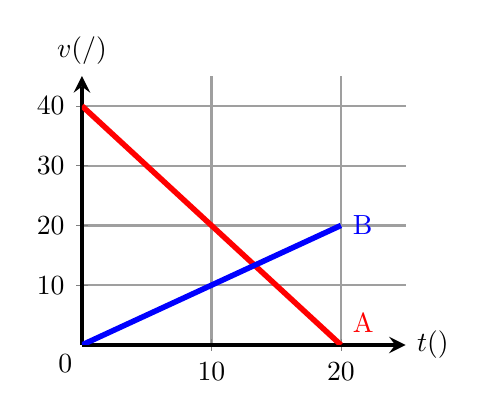
\begin{tikzpicture}  
		\begin{axis}[  ultra thick,scale=0.6,
			xmin=0,  
			xmax=25,  
			xtick={0,10,20},
			ytick={0,10,...,40},
			minor x tick num=0,
			minor y tick num=0,
			ymin=0,  
			ymax=45, 
			samples=300,
			axis lines=center, 
			grid style={step=1, line width =0.4pt, color=gray!40!white},
			grid=both, %giới hạn ô lưới
			major grid style={line width=0.8pt,gray!75!white},
			xlabel=$\xsi{t}{\left(\si{\second}\right)}$, 		ylabel=$\xsi{v}{\left(\si{\meter/\second}\right)}$,
			every axis y label/.style={at=(current axis.above origin),anchor=south},  
			every axis x label/.style={at=(current axis.right of origin),anchor=west},  ]
			\addplot [line width=2pt, red, smooth, domain=0:20] {40-2*x} node[above right] {A}; 
			\addplot [line width=2pt, blue, smooth, domain=0:20] {x} node[right] {B};  
			\coordinate (O) at (axis cs: 0,0);
		\end{axis}  
		\node[below left] at (O) {0};
	\end{tikzpicture}
	}
	\loigiai{}
\end{ex}
% ======================================================================
\begin{ex}
	Một người đứng ở sân ga nhìn ngang đầu toa tàu thứ nhất của một đoàn tàu bắt đầu chuyển bánh. Thời gian toa thứ nhất qua trước mặt người ấy là $t_1=\SI{6}{\second}$. Hỏi toa thứ 7 qua trước mặt người ấy trong bao lâu? Biết rằng đoàn tàu chuyển động thẳng nhanh dần đều, chiều dài các toa bằng nhau và khoảng hở giữa 2 toa là không đáng kể.
	\loigiai{}
\end{ex}
\Closesolutionfile{ans}
\begin{center}
	\textbf{-- HẾT --}
\end{center}